
\section{Создание экспериментального образца}

\subsection{Сборка квадрокоптера}
На основе компонентов, указанных в главе "Разработка архитектуры микродрона" собирается квадрокоптер. К раме прикручиваются плата регуляторов и моторы. Фазы каждого мотора припаиваются на соответствующие площадки регуляторов. При проверке вращения моторов в случае несоответствия вращения мотора схеме для px4, необходимо перепаять любые две фазы этого мотора. Также к регуляторам припаиваются силовые провода с коннектором для подключения аккумулятора. Ставится поверх регулятора полетный контроллер, он подключается к регуляторам через колодку. Далее производится монтаж FPV оборудования, приемника и телеметрийного модуля. (рис. \ref{fig:quad1}).
% ~\ref{fig:quad1}
\begin{figure}[H]
	\centering
	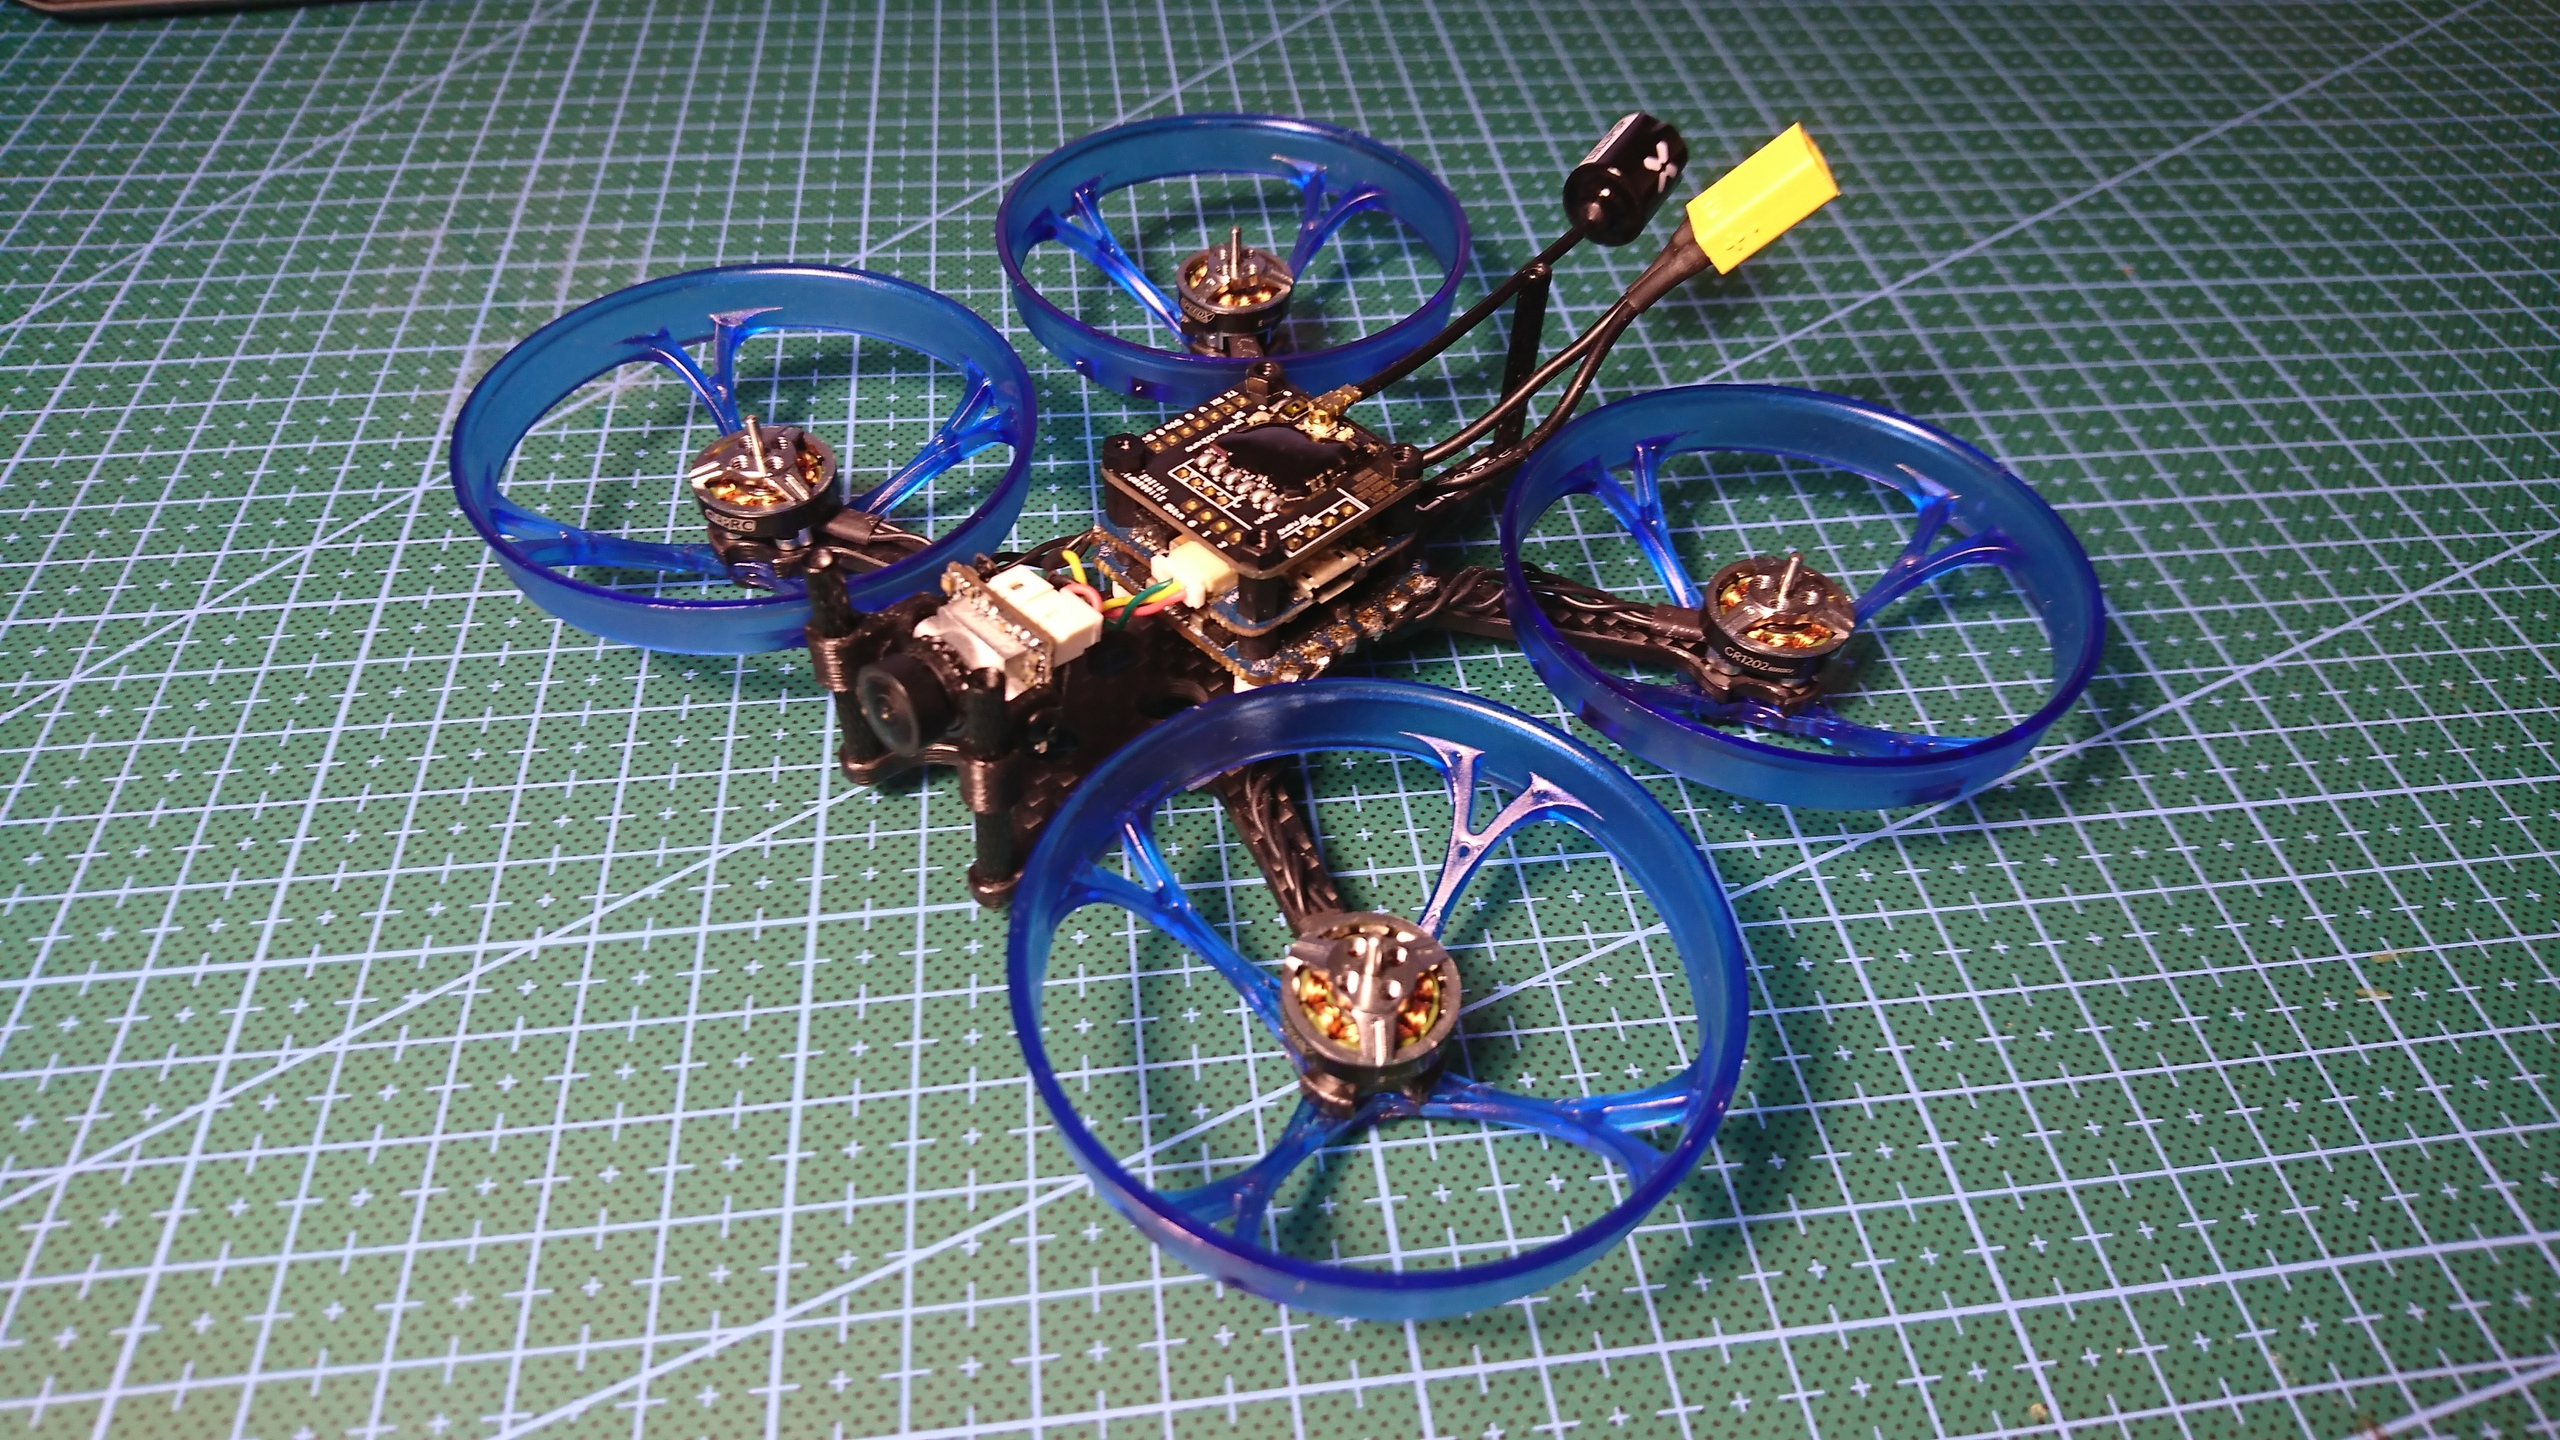
\includegraphics[width=0.5\linewidth]{pics/quad1}
	\caption{Установка компонентов на раму
	}
	\label{fig:quad1}
\end{figure}
Прикручивается верхняя пластина рамы, закрепляются все свисающие детали и на этом сборка завершается (рис. \ref{fig:quad2}).
% ~\ref{fig:quad2}
\begin{figure}[H]
	\centering
	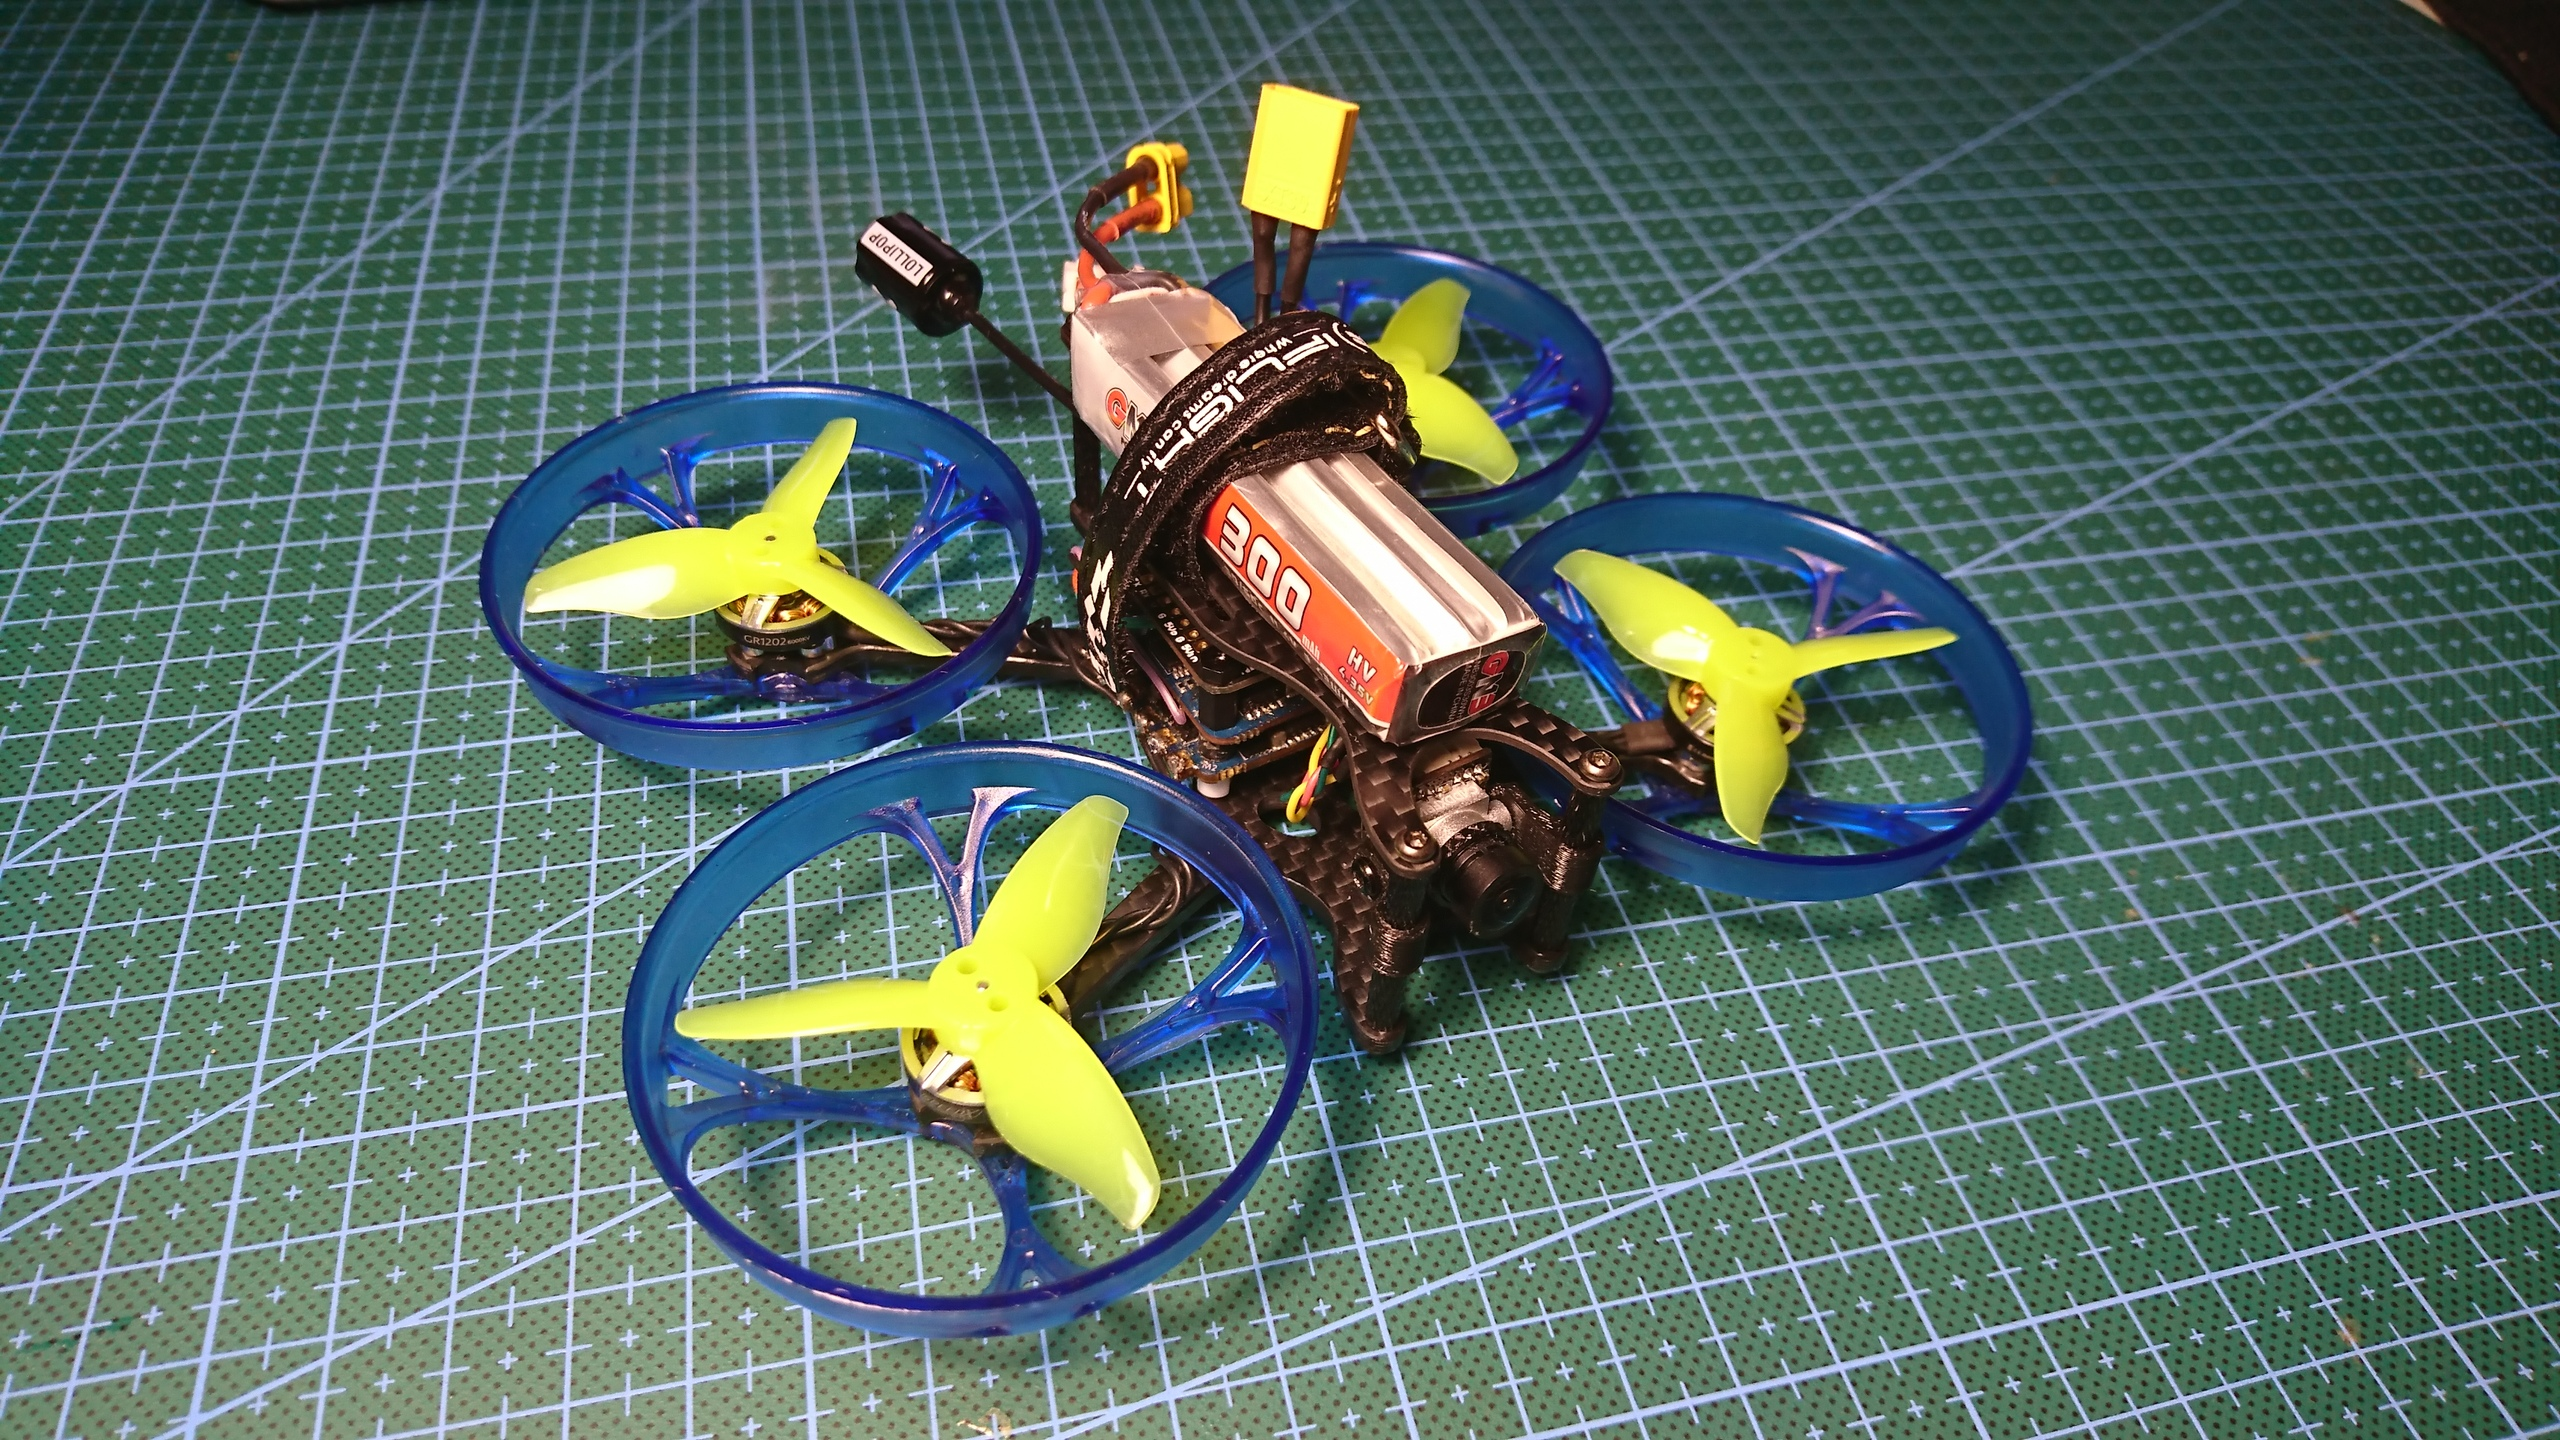
\includegraphics[width=0.5\linewidth]{pics/quad2}
	\caption{Экспериментальный образец квадрокоптера
	}
	\label{fig:quad2}
\end{figure}

\subsection{Сборка наземной станции}
Согласно шагам из главы "Разработка архитектуры наземной станции" производится сборка наземной станции.
\subsection{Обновление и настройка параметров ПО}
На полетный контроллер через qgroundcontrol по USB прошивается последний образ PX4. Производится калибровка всех датчиков. Для взаимодействия приемника с радиомодулем требуется привязка посредством нажатия кнопки bind.
Настраиваются бод -- рейты устройств приема -- передачи телеметрии на максимально доступное значение. Для экспериментального образца использовались устройства 3DR с бод -- рейтами 115200. При подключении через 3DR модули параметры квадрокоптера считались и отобразились в конфигураторе. Остается настройка базовой станции. Настраивается видеоприемник на диапазон частот видеопередатчика. Окружение для наземной станции создавалось на базе пакета clover, где предустановлены все необходимые инструменты. В launch файлах меняются параметры для способа подключения, чтобы была доступна симуляция окружения квадрокоптера. Для топика указывается порт, к которому подключен видеомодуль. После перезагрузки применяются параметры и можно приступать к тестированию.
\subsection{Проверка работы экспериментального образца}
Для проверки работы aruco\_detect создается карта маркеров, прописанная в конфигурационном файле пакета clover (рис. \ref{fig:map}).
% ~\ref{fig:map}
\begin{figure}[H]
	\centering
	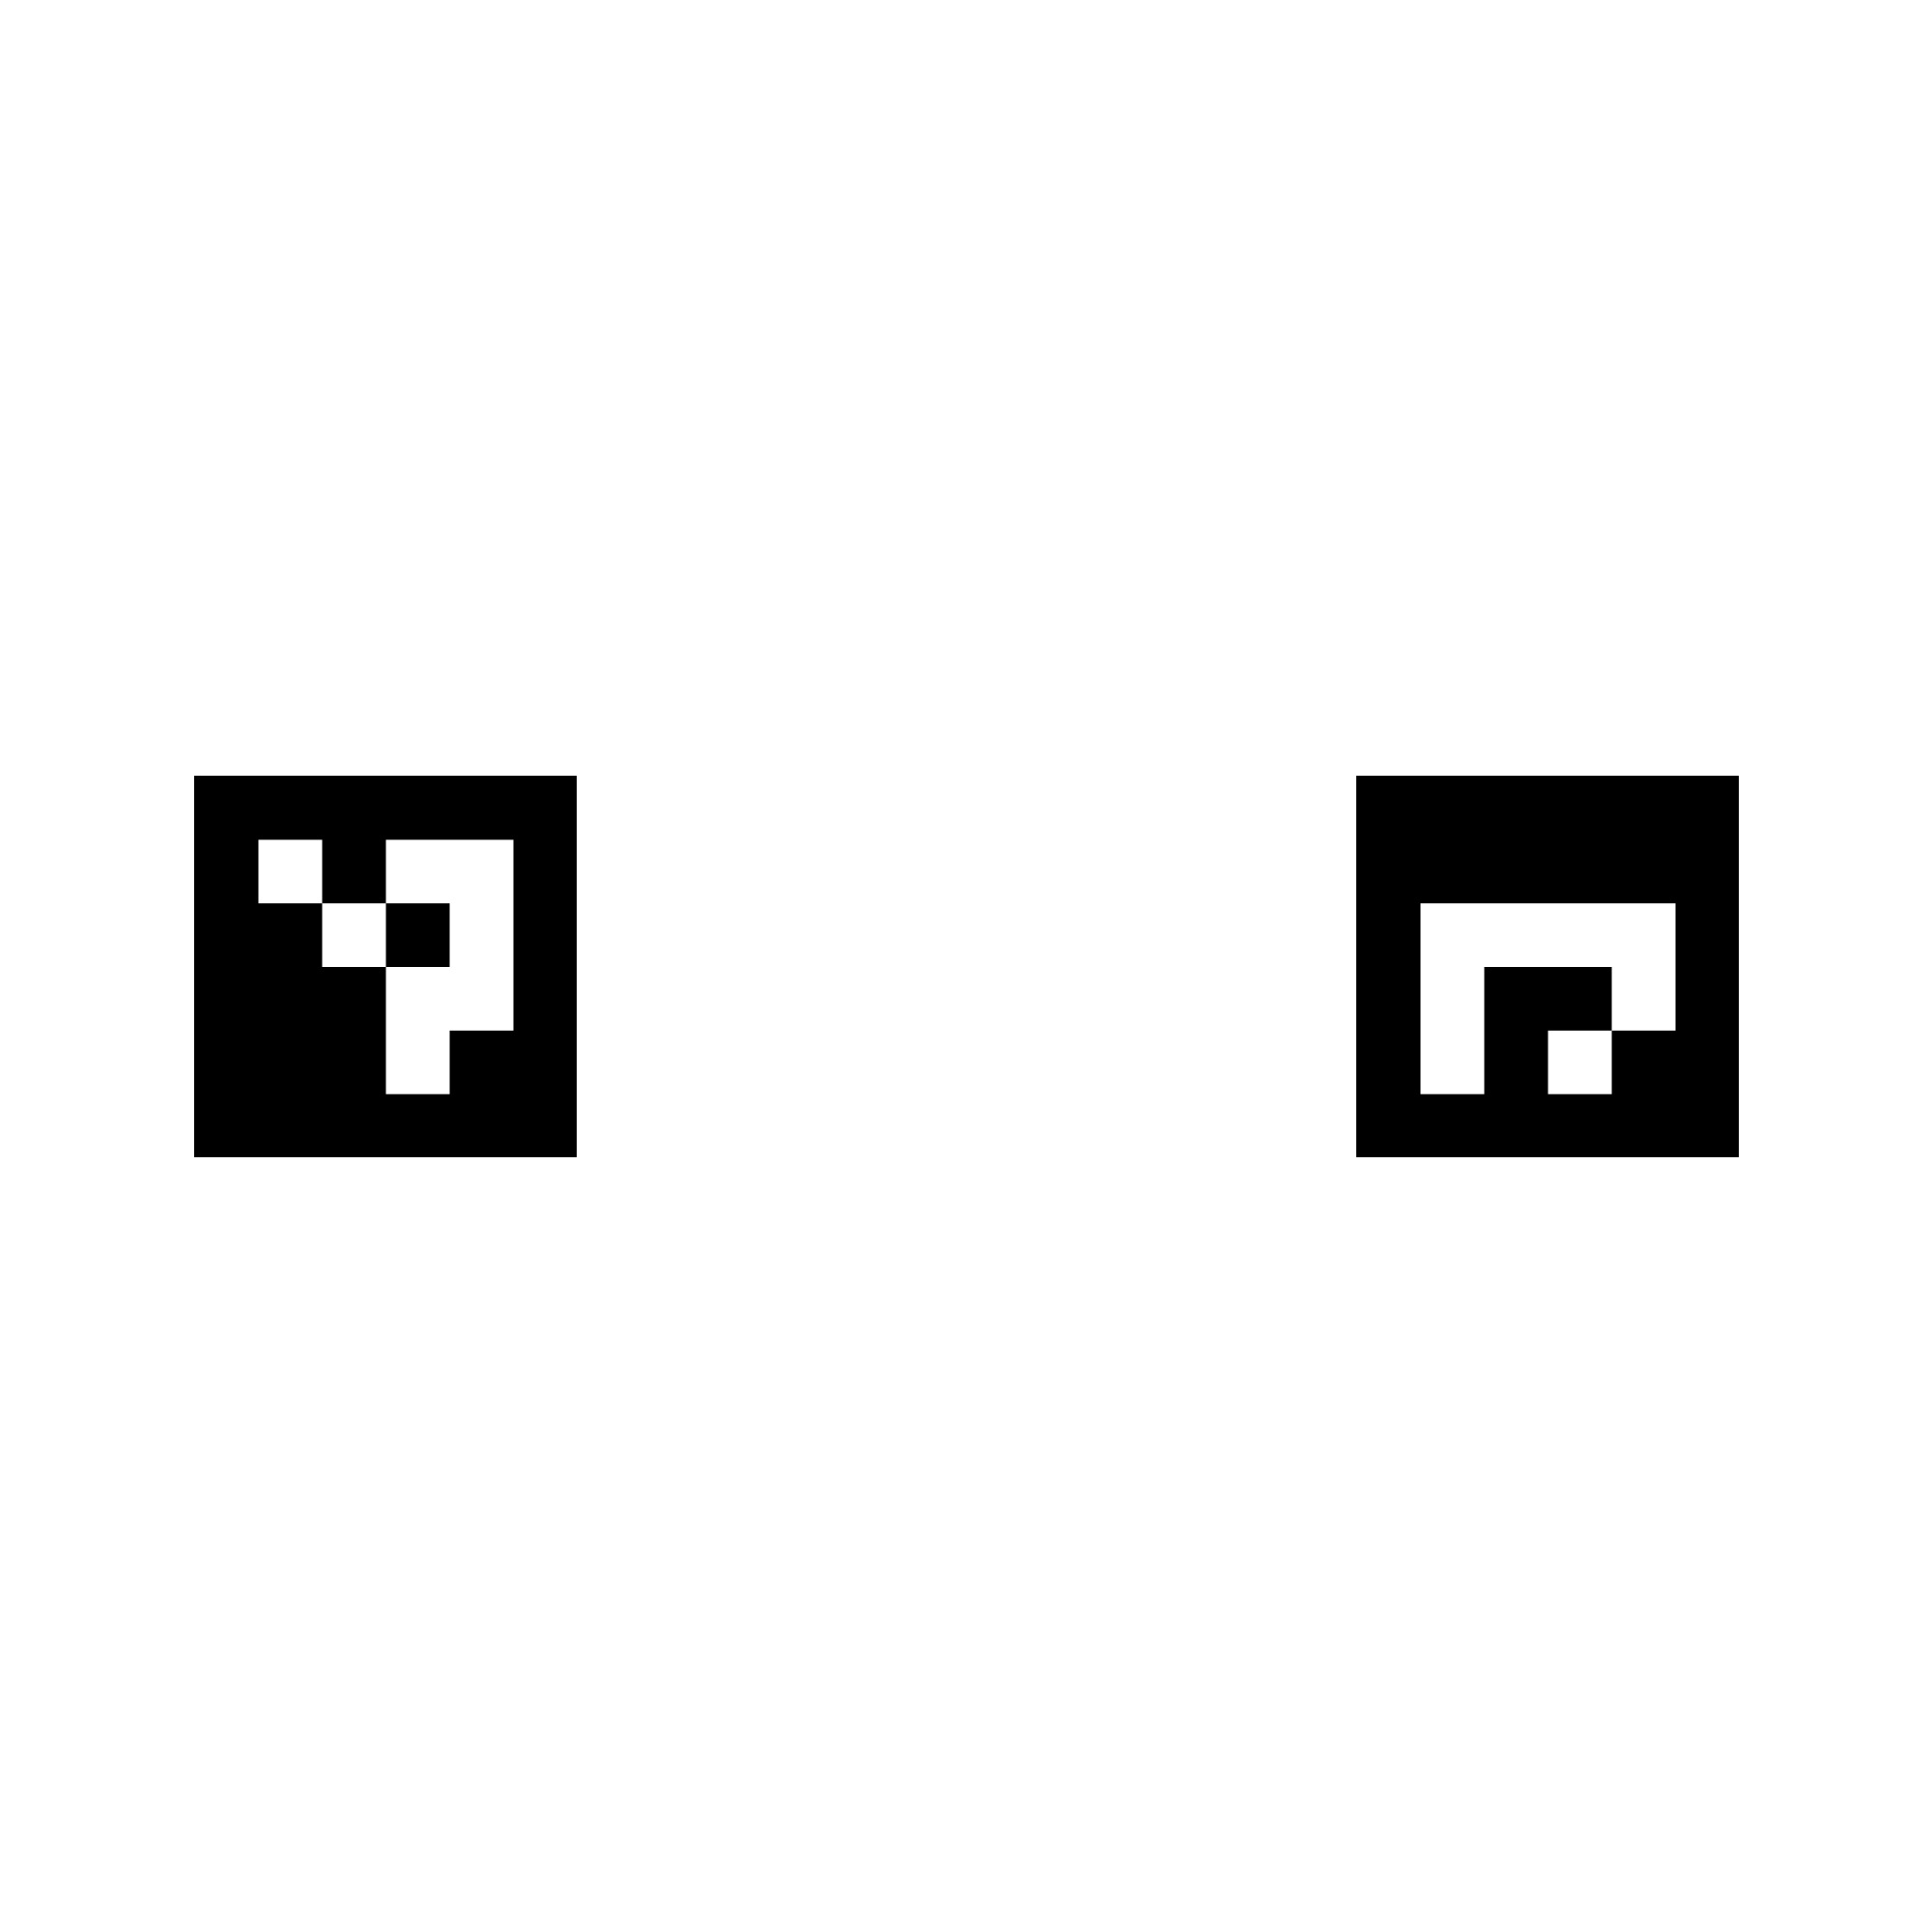
\includegraphics[width=0.5\linewidth]{pics/map}
	\caption{Карта маркеров
	}
	\label{fig:map}
\end{figure}
Наводим камеру квадрокоптера на метки, проверяем топик aruco\_detect и получаем идентификаторы меток (рис. \ref{fig:aruco_detect}).
% ~\ref{fig:aruco_detect}
\begin{figure}[H]
	\centering
	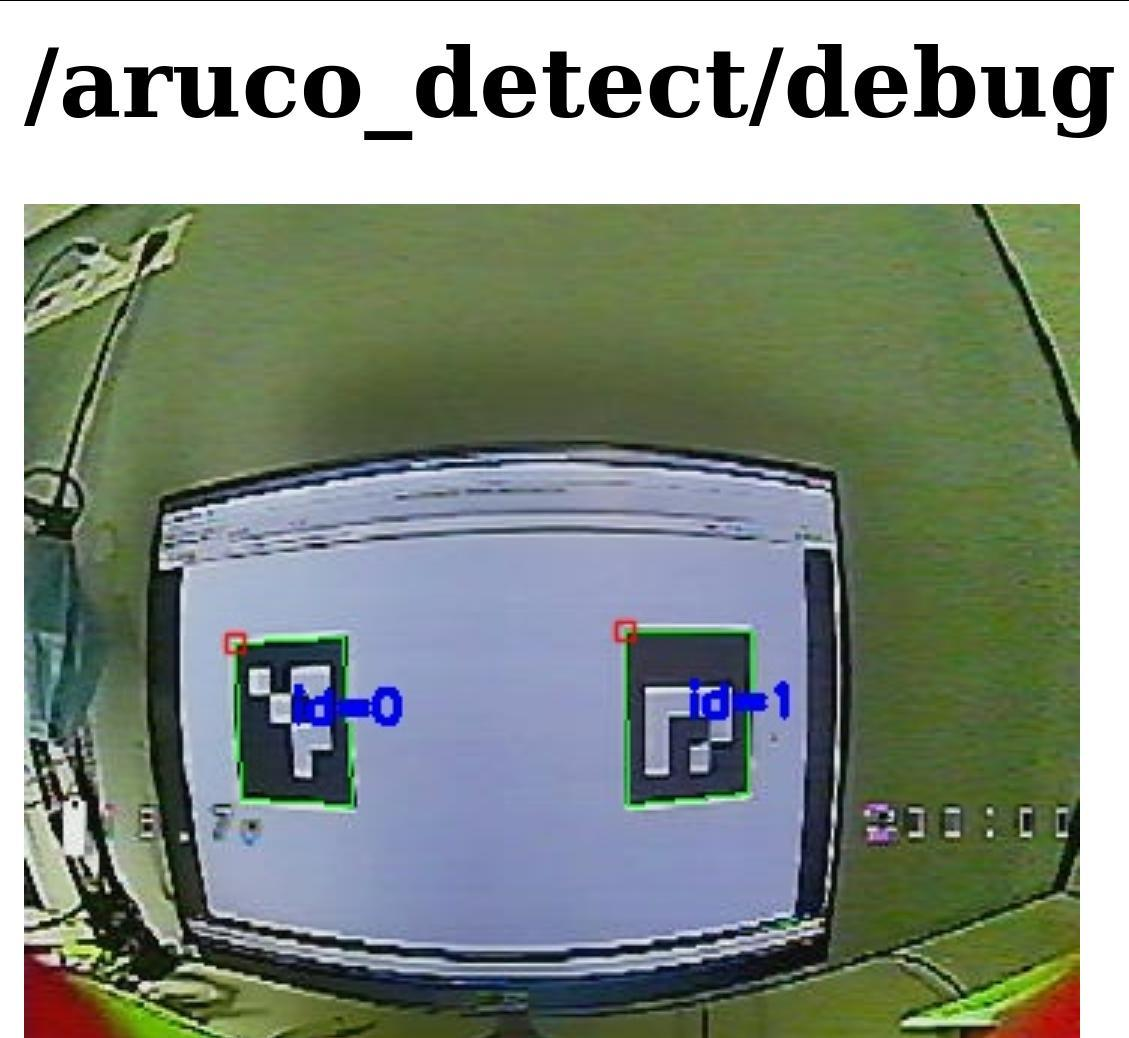
\includegraphics[width=0.5\linewidth]{pics/aruco_detect}
	\caption{Инициализация aruco маркеров
	}
	\label{fig:aruco_detect}
\end{figure}
Замеряем задержку (рис. \ref{fig:time}).
% ~\ref{fig:time}
\begin{figure}[H]
	\centering
	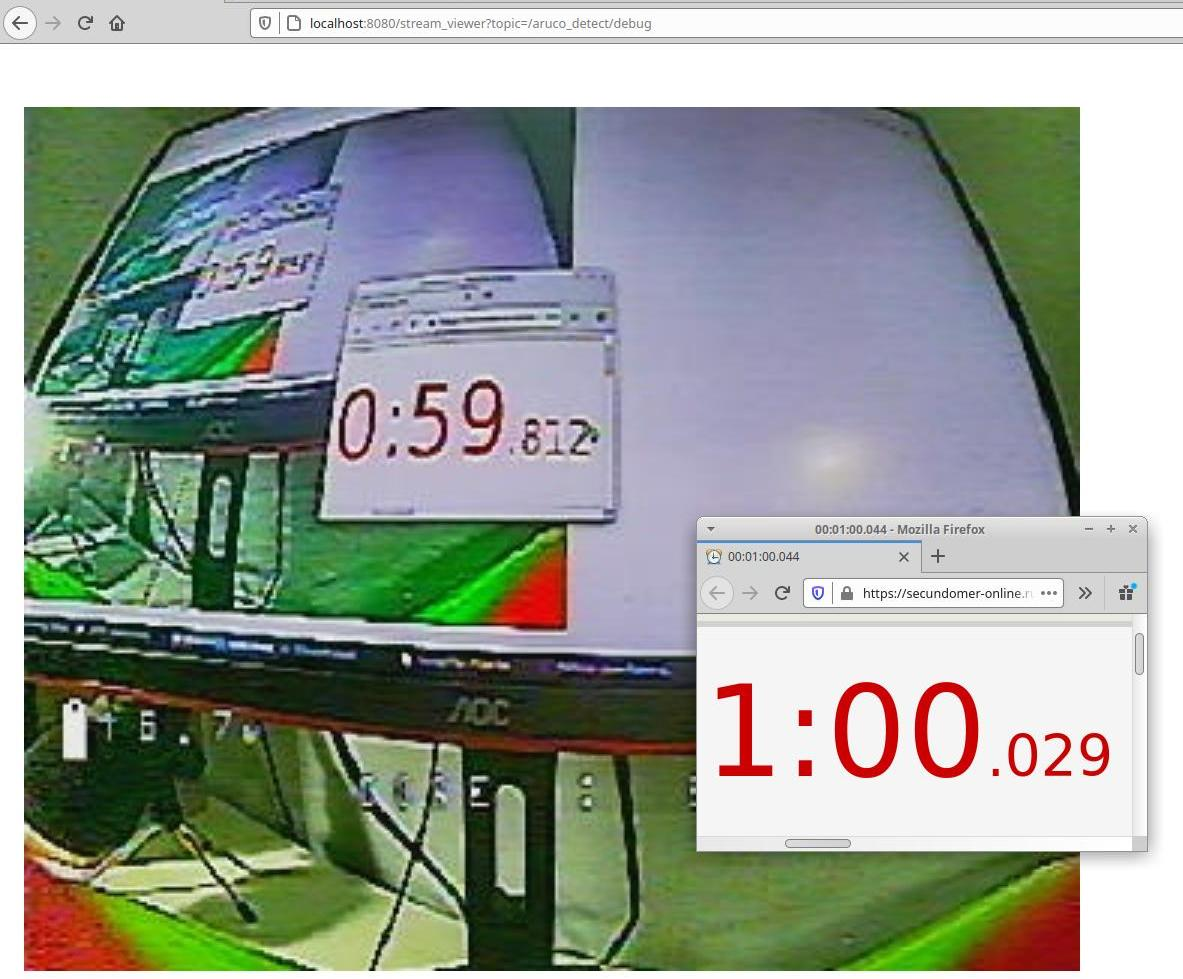
\includegraphics[width=0.5\linewidth]{pics/time}
	\caption{Время задержки% 0.2с
	}
	\label{fig:time}
\end{figure}
200 мс - критичное значение, появившееся в сумме задержек каждого устройства (камеры, видеопередатчика, видеоприемника, USB порта компьютера). Учитывая, что задержка также присутствует на устройстве приема -- передачи телеметрии, обнаруживается критичная проблема у разрабатываемого комплекта. Для уменьшения задержки при получении -- передаче телеметрии необходим бод -- рейт 921600. Для уменьшения задержки получения видеопотока необходимо изучить другие системы передачи видеопотока, например, OpenHD \cite{openhd}.

